% !TEX ROOT=./main.tex

\section{Details on Experiments and Additional Results}
% \subsection{Experiments}
\label{sec:expsupp}

We described the precise procedure to reproduce the results in this paper.
As we mentioned in Section~\ref{sec:exp}, we empirically verified the
linear speed up on various convex settings for both FedAvg and its
accelerated variants. For all the results, we set random seeds as $0, 1, 2$
and report the best convergence rate across the three folds. For each
run, we initialize $\vw_0 = \mathbf{0}$ and measure the number of iteration
to reach the target accuracy $\epsilon$. We use the small-scale dataset
w8a~\cite{platt1998fast}, which consists of $n = 49749 $ samples with
feature dimension $d = 300$. The label is either positive one or negative one.
The dataset has sparse binary features in $\{0, 1\}$. Each sample
has 11.15 non-zero feature values out of $300$ features on average.
We set the batch size equal to four across all experiments.
In the next following subsections,
we introduce parametering searching in each objective separately.


\subsection{Strongly Convex Objectives}
We first consider the strongly convex objective function, where we use
a regularized binary logistic regression with regularization $\lambda=1/n\approx 2e-5$. We evenly distributed on $1, 2, 4, 8, 16, 32$ devices and  report the number of iterations/rounds needed to converge to $\epsilon-$accuracy, where $\epsilon=0.005$. The optimal objective function value $f^*$
is set as $f^* = 0.126433176216545$. This is determined numerically and we follow the setting in~\cite{stich2018local}. The learning rate is decayed as the $\eta_t = \min(\eta_0, \frac{nc}{1 + t})$, where we extensively search the best learning rate $c \in \{2^{-1}c_0, 2^{-2}c_0, c_0, 2c_0, 2^{2}c_0\}$. In this case, we search the initial learning rate $\eta_0\in \{1, 32\}$ and $c_0 = 1/8$.


\subsection{Convex Smooth Objectives}
We also use binary logistic regression without regularization.
The setting is almost same as its regularized counter part. We also evenly distributed all the samples on $1, 2, 4, 8, 16, 32$ devices. The figure shows the number of iterations needed to converge to $\epsilon-$accuracy, where $\epsilon=0.02$. The optiaml objective function value is set as $f^*=0.11379089057514849$, determined numerically. 
The learning rate is decayed as the $\eta_t = \min(\eta_0, \frac{nc}{1 + t})$, where we extensively search the best learning rate $c \in \{2^{-1}c_0, 2^{-2}c_0, c_0, 2c_0, 2^{2}c_0\}$. In this case, we search the initial learning rate $\eta_0\in \{1, 32\}$ and $c_0 = 1/8$.


\subsection{Linear regression}
For linear regression, we use the same feature vectors from w8a dataset 
and generate ground truth $[\vw^*, b^*]$ from a multivariate normal distribution
with zero mean and standard deviation one. Then we generate label 
based on $y_i = \vx_i^t\vw^* + b^*$. This procedure will ensure we satisfy
the over-parameterized setting as required in our theorems. 
We also evenly distributed all the samples on $1, 2, 4, 8, 16, 32$ devices. The figure shows the number of iterations needed to converge to $\epsilon-$accuracy, where $\epsilon=0.02$. The optiaml objective function value is $f^*=0$. 
The learning rate is decayed as the $\eta_t = \min(\eta_0, \frac{nc}{1 + t})$, where we extensively search the best learning rate $c \in \{2^{-1}c_0, 2^{-2}c_0, c_0, 2c_0, 2^{2}c_0\}$. In this case, we search the initial learning rate $\eta_0\in \{0.1, 0.12\}$ and $c_0 = 1/256$.

\subsection{Partial Participation}
To examine the linear speedup of FedAvg in partial participation experiments,
we evenly distributed data on $4, 8, 16, 32, 64, 128$ devices and 
uniformly sample $50\%$ devices without replacement. All other hyperparameters
are the same as previous sections. 

\subsection{Nesterov accelerated FedAvg}
The experiments of Nesterov accelerated FedAvg (the update formula is given as follows) uses the same setting as
previous three sections for vanilia FedAvg.
\begin{align*}
\vy_{t+1}^{k} & =\vw_{t}^{k}-\alpha_{t}\vg_{t,k}\\
\vw_{t+1}^{k} & =\begin{cases}
\vy_{t+1}^{k}+\beta_{t}(\vy_{t+1}^{k}-\vy_{t}^{k}) & \text{if }t+1\notin\mathcal{I}_{E}\\
\sum_{k\in\mathcal{S}_{t+1}}\left(\vy_{t+1}^{k}+\beta_{t}(\vy_{t+1}^{k}-\vy_{t}^{k})\right) & \text{if }t+1\in\mathcal{I}_{E}
\end{cases}
\end{align*}
We set $\beta_t = 0.1$ and search $\alpha_t$ in the same way as $\eta_t$
in FedAvg.


\subsection{The impact of $E$.}
In this subsection, we further examine how does the number of local steps ($E$) 
affect convergence. As shown in Figure~\ref{fig:e}, the number of iterations increases as $E$ increase, which slow down the convergence in
terms of gradient computation. However, it can save communication costs as
the number of rounds decreased when the $E$ increases. This showcase that
we need a proper choice of $E$ to trade-off the communication cost and
convergence speed. 
\begin{figure}
\centering
	\begin{tabular}{ccc}
	\hspace{-2em} 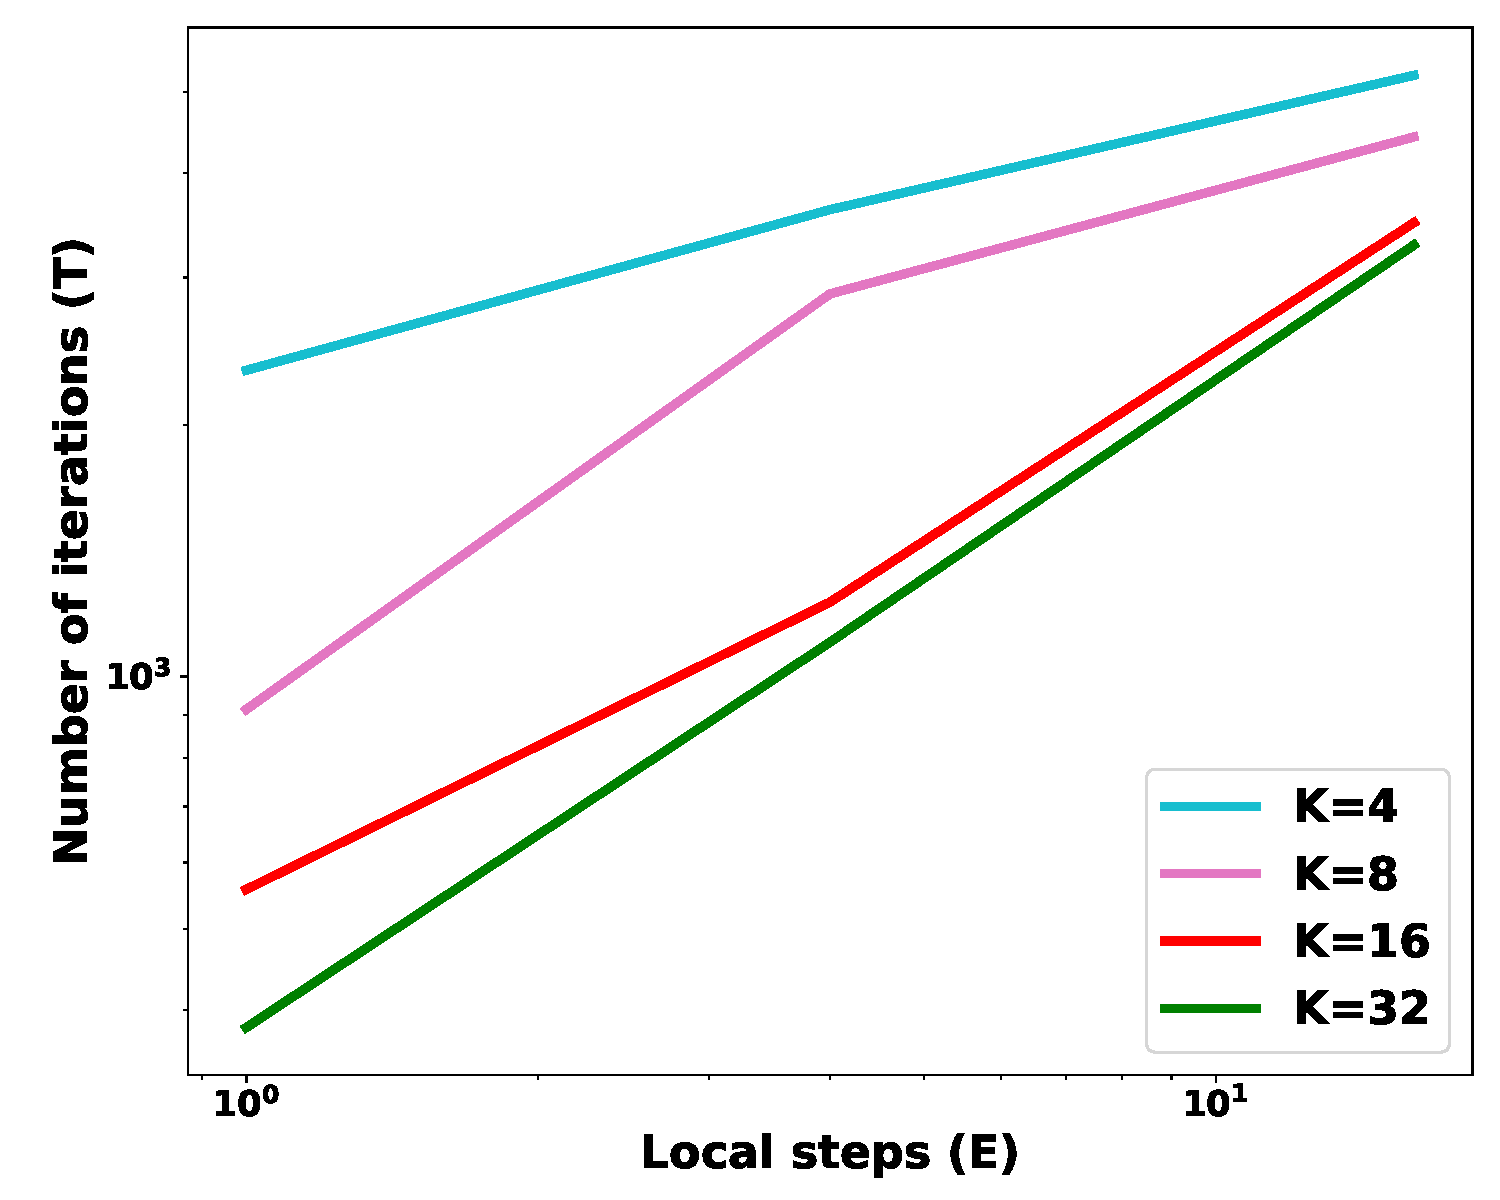
\includegraphics[width=0.33\textwidth]{fig/paper-stronglycvxsmthspeedupEpochsT-min-w8a-epsilon0131-reg1e-05.pdf} &
	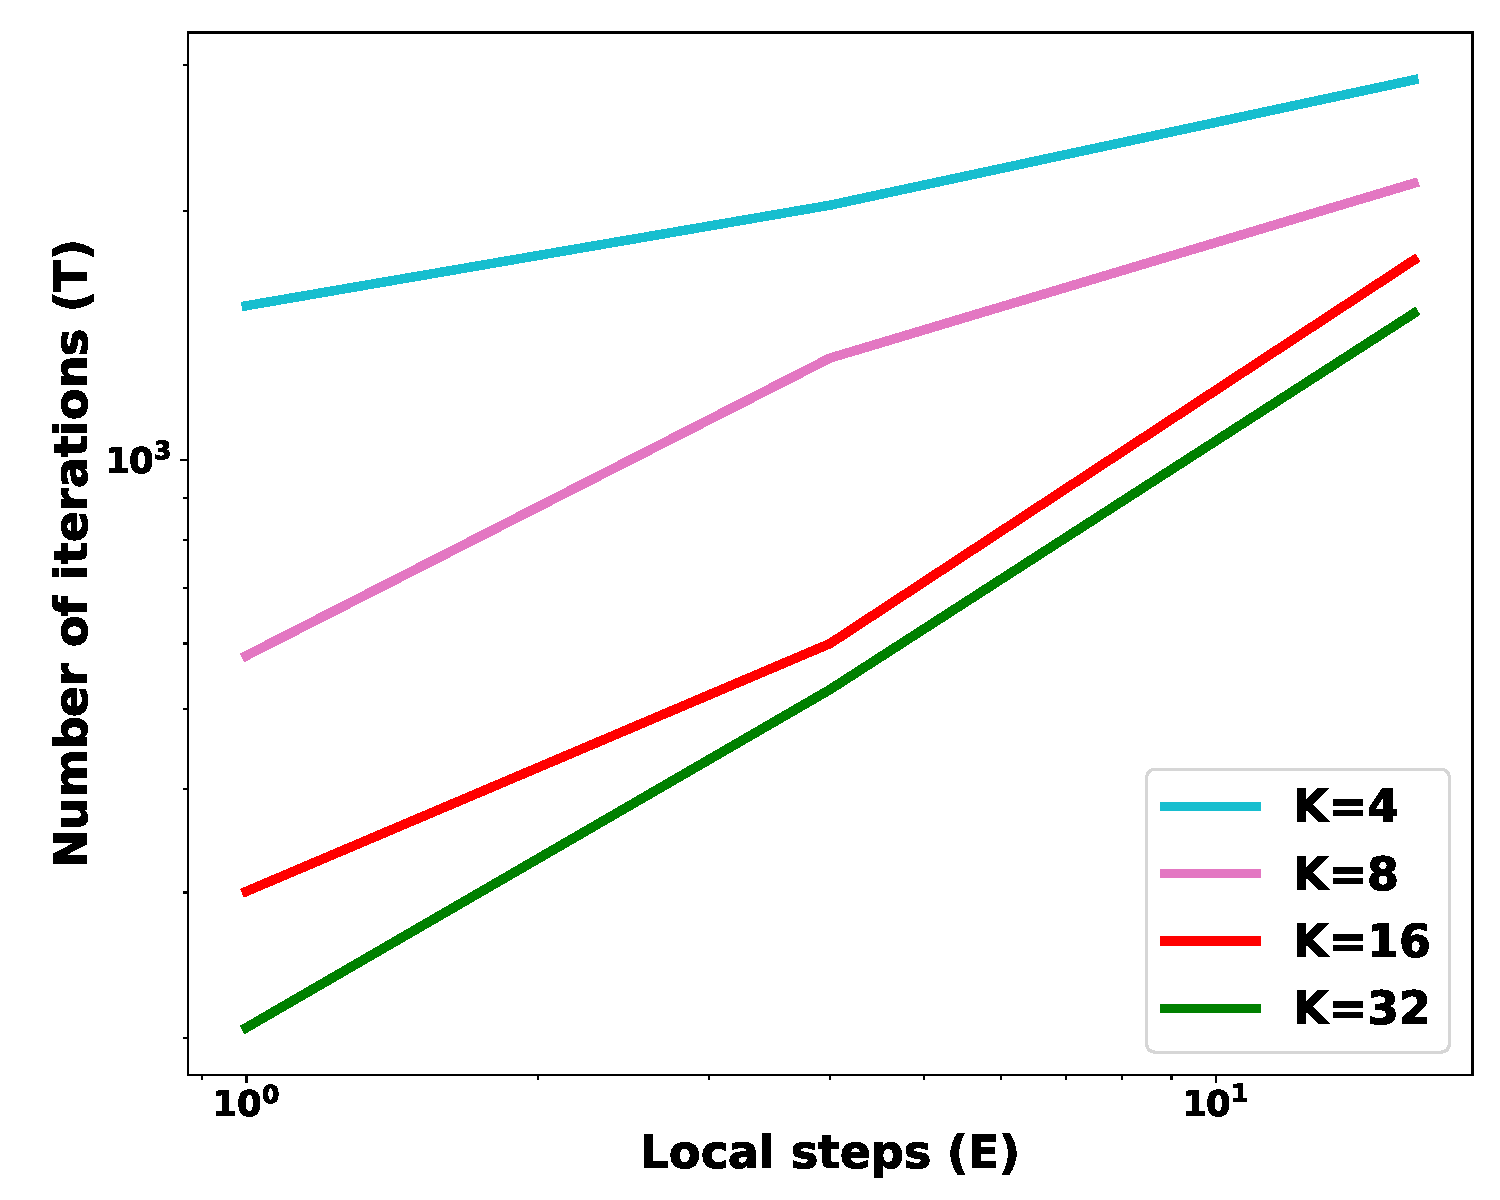
\includegraphics[width=0.33\textwidth]{fig/paper-cvxsmoothspeedupEpochsT-min-w8a-epsilon0134-reg0.pdf} & 
	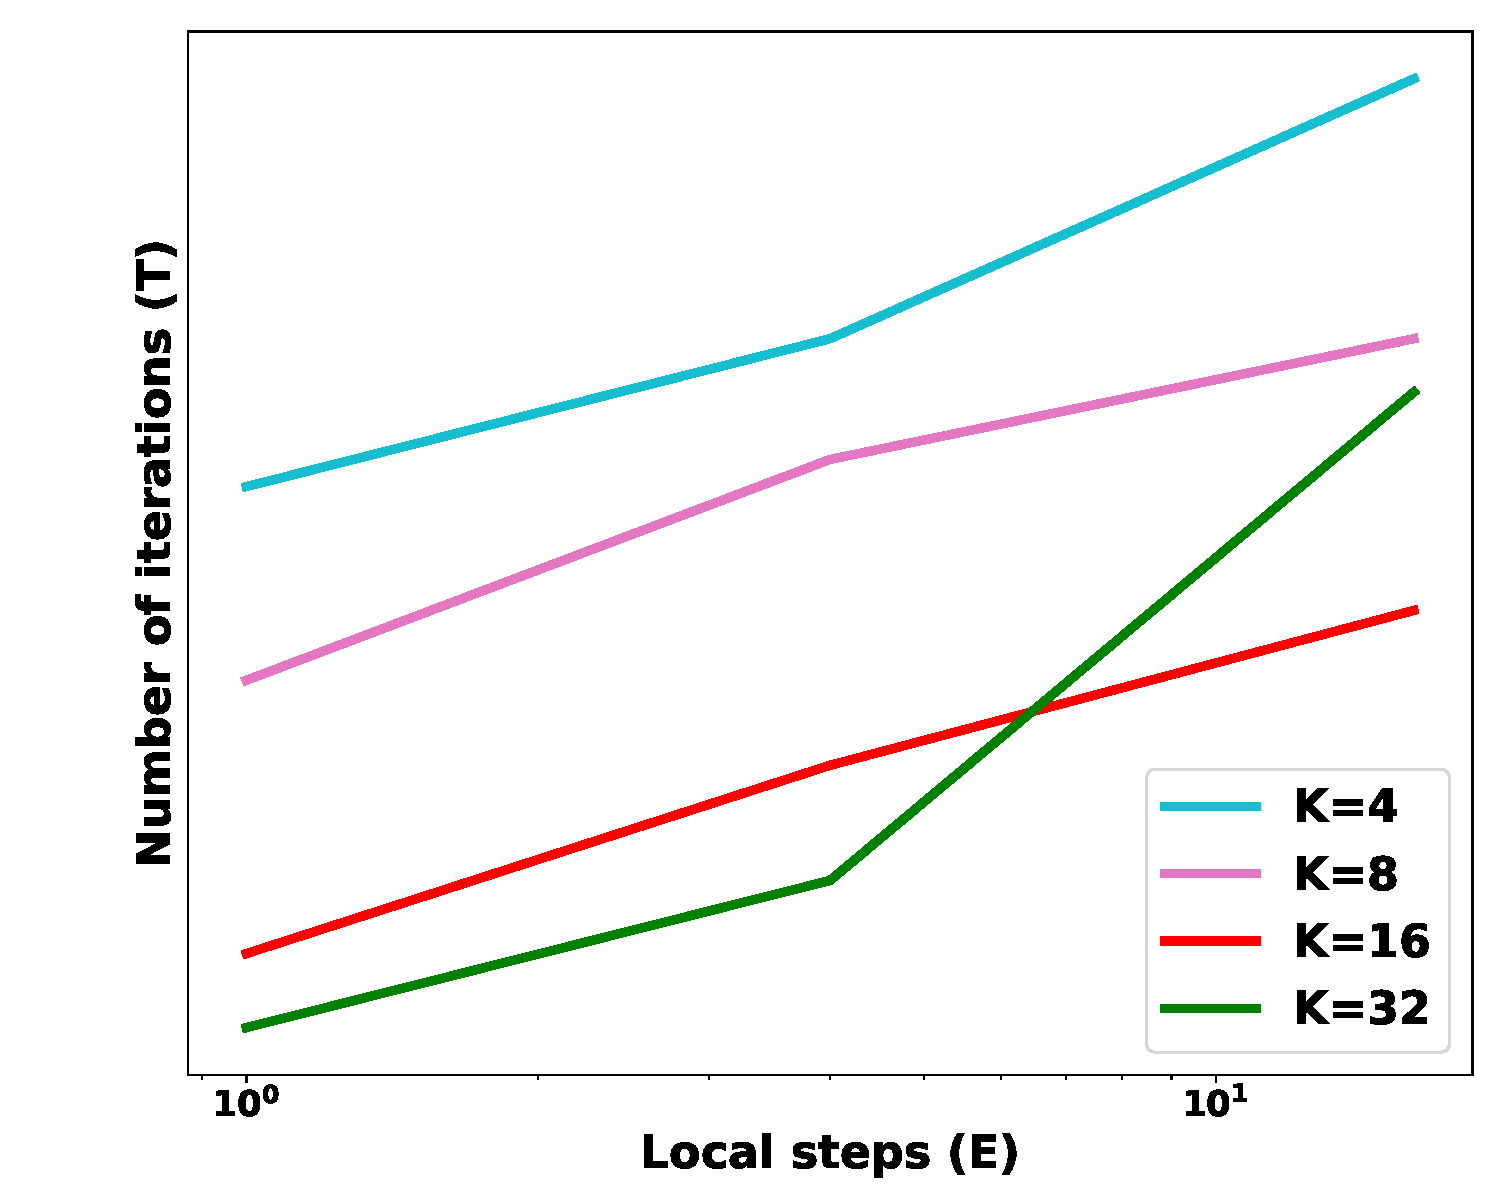
\includegraphics[width=0.33\textwidth]{fig/paper-linregression-newspeedupEpochsT-min-linearregressionw8a-epsilon002-reg0.pdf} \\
	\hspace{-2em} 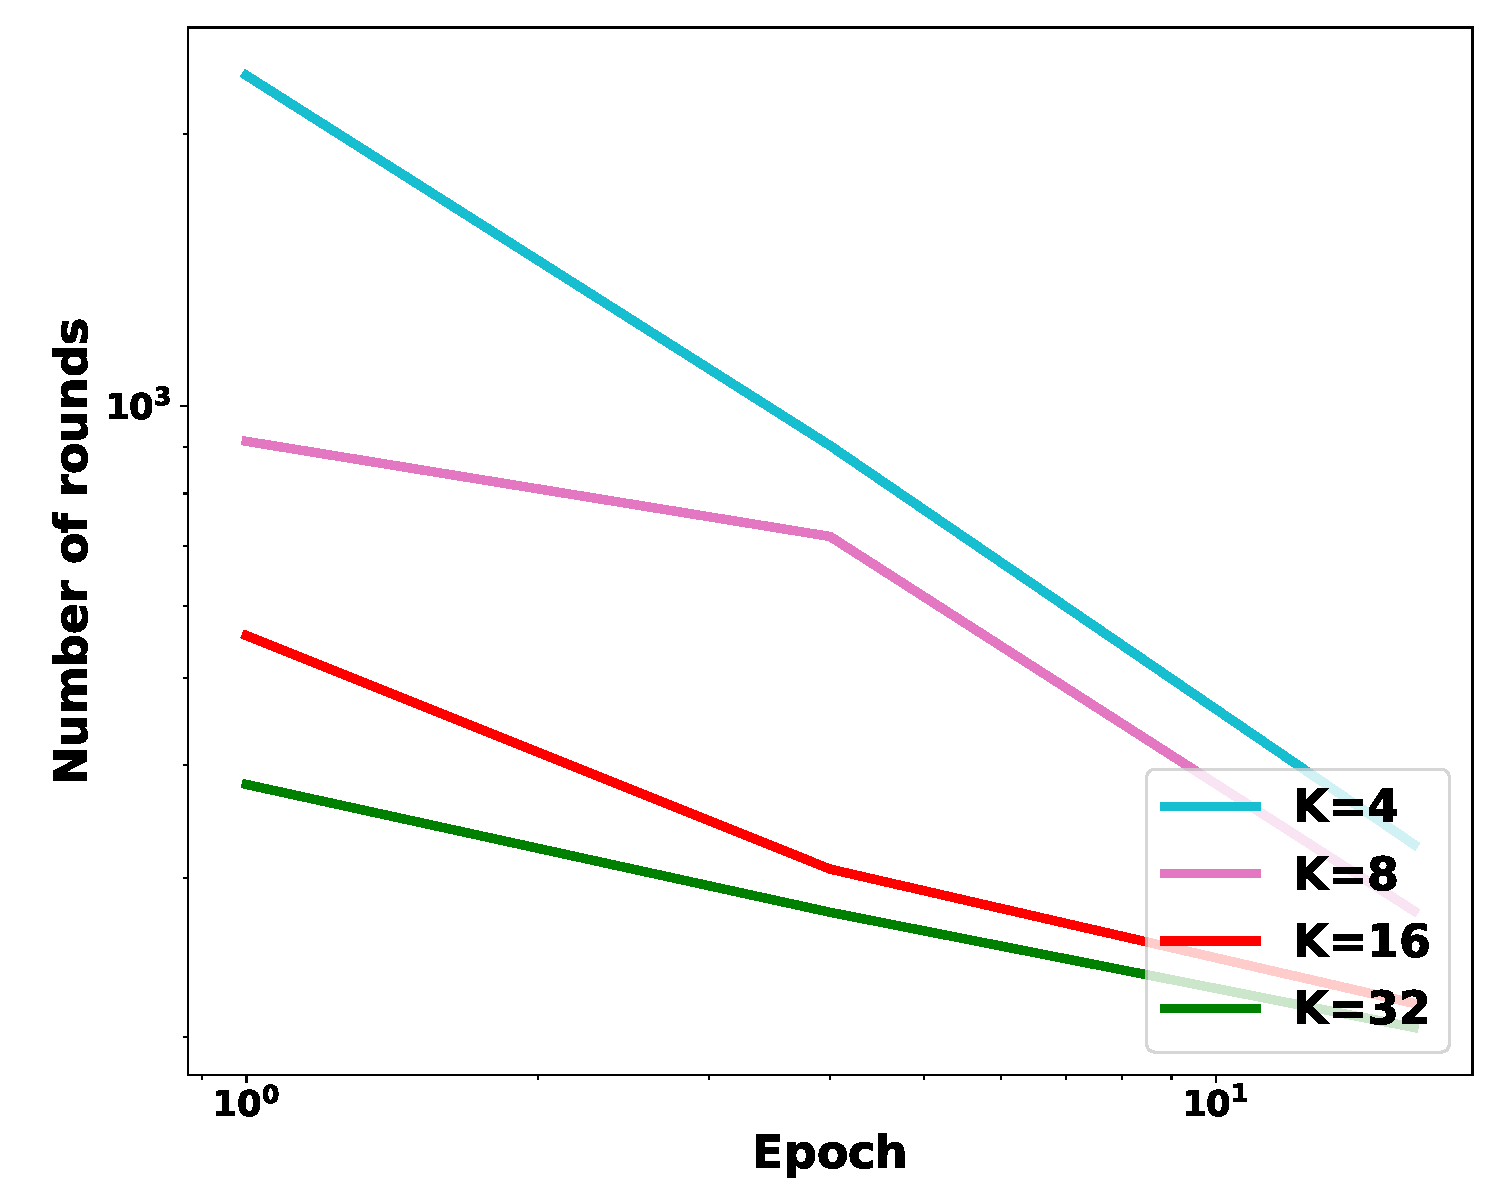
\includegraphics[width=0.33\textwidth]{fig/paper-stronglycvxsmthspeedupEpochsRounds-min-w8a-epsilon0131-reg1e-05.pdf} &
	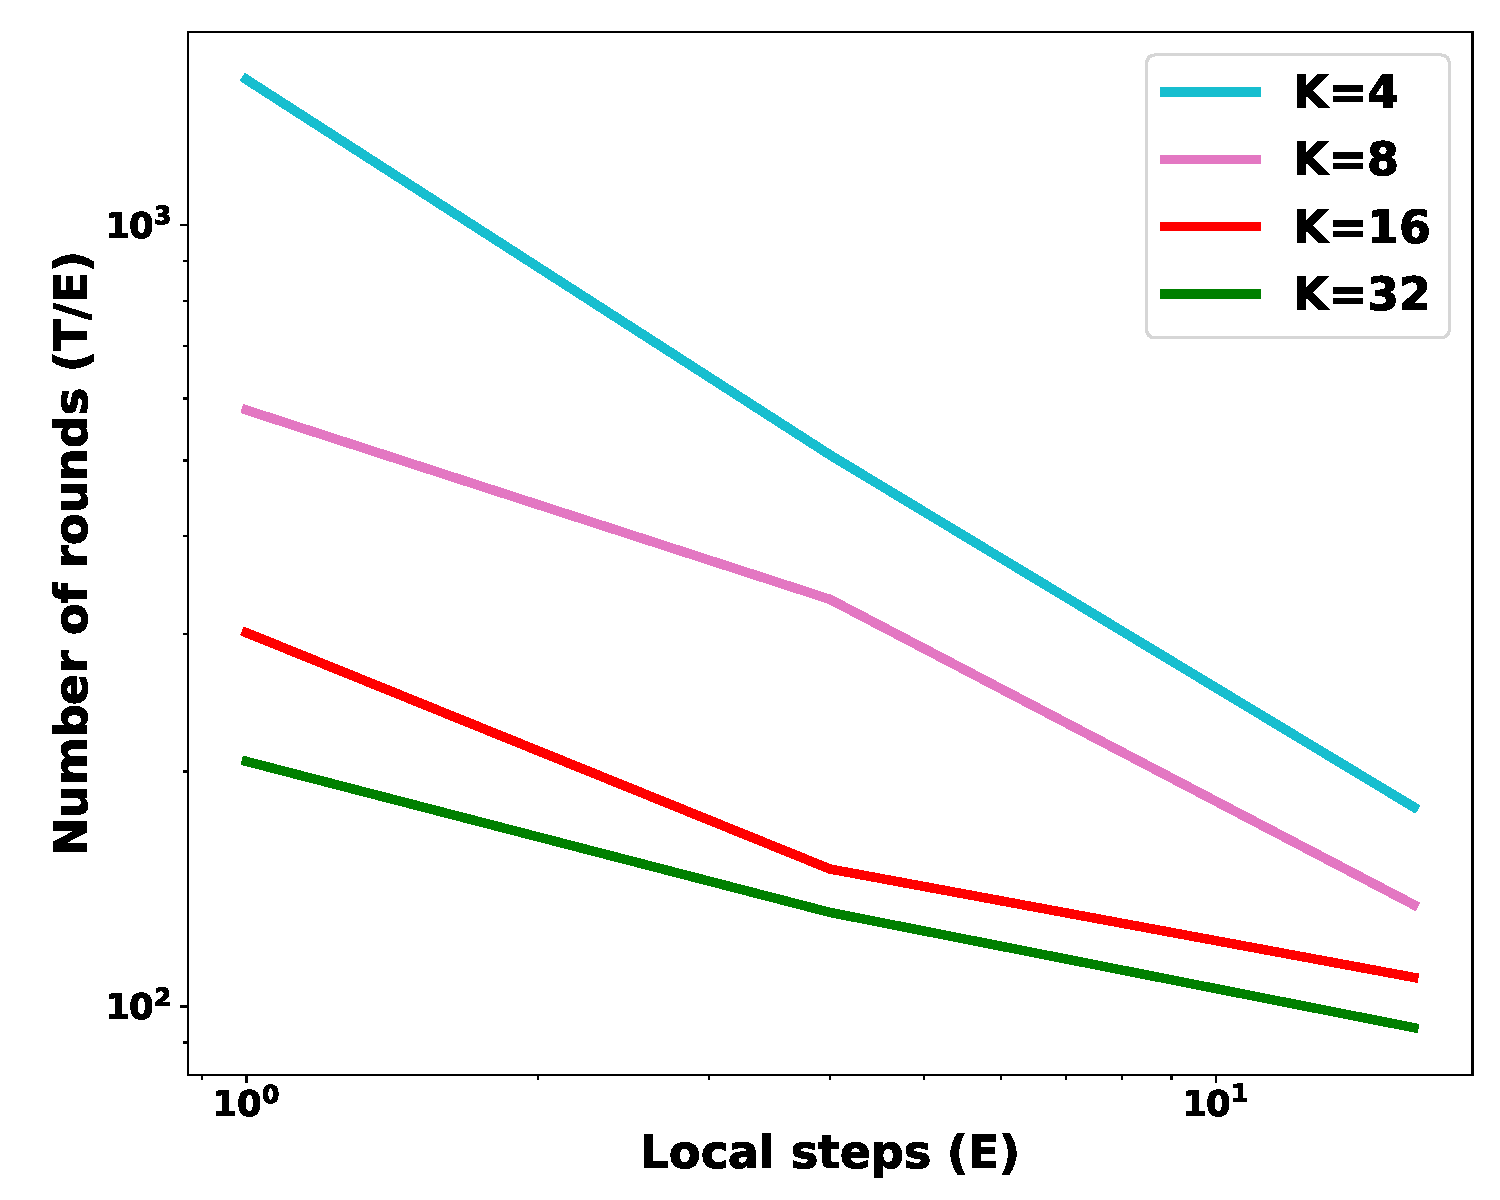
\includegraphics[width=0.33\textwidth]{fig/paper-cvxsmoothspeedupEpochsRounds-min-w8a-epsilon0134-reg0.pdf} & 
	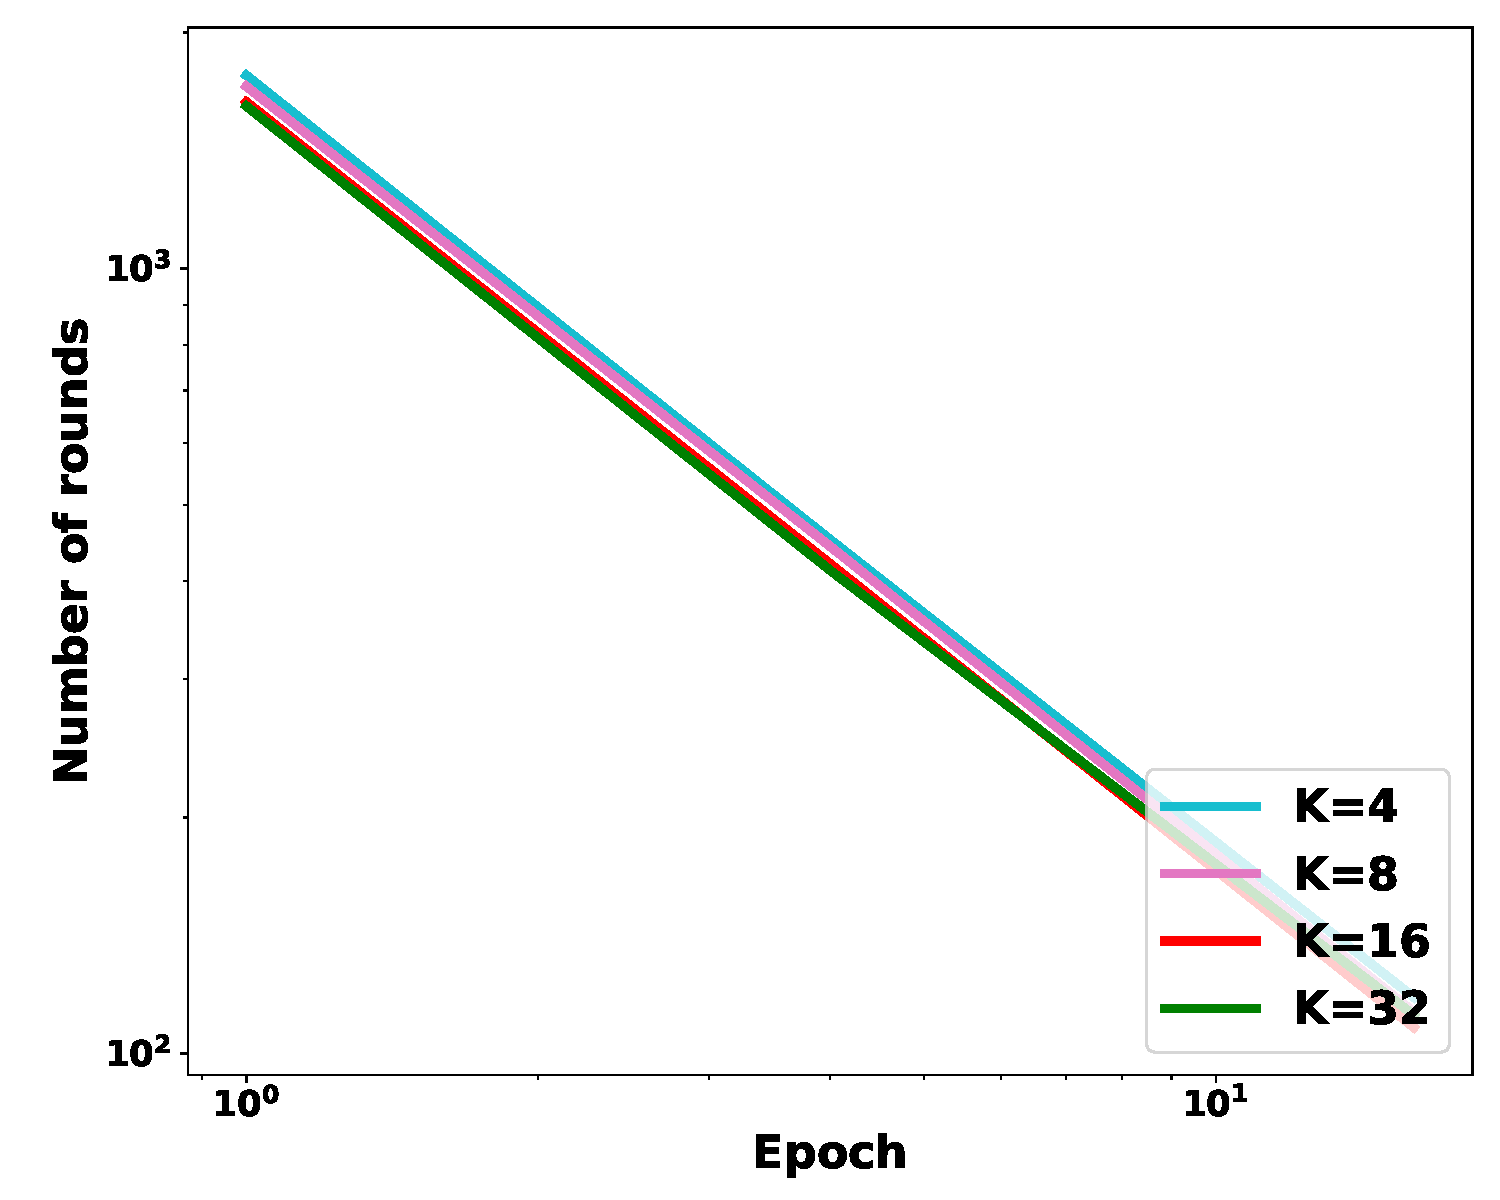
\includegraphics[width=0.33\textwidth]{fig/paper-linregression-newspeedupEpochsRounds-min-linearregressionw8a-epsilon002-reg0.pdf} \\
(a) Strongly convex objective & (b) Convex smooth objective & (c) Linear regression
	\end{tabular}
\caption{The convergence of FedAvg w.r.t the number of local steps $E$. }
\label{fig:e}
\end{figure}

